\documentclass[compress, red]{beamer}
\usepackage[utf8]{inputenc}
\usepackage[english, russian]{babel}

\usetheme{CambridgeUS}
\usecolortheme{default}
\useoutertheme[subsection=false]{smoothbars}

\usepackage{framed}
\usepackage[pages=some]{background}
\usepackage[T2A]{fontenc}
\usepackage[utf8]{inputenc}
\usepackage[russian]{babel}

\hypersetup{
    colorlinks=true,
    linkcolor=black,
    filecolor=magenta,      
    urlcolor=cyan,
    pdftitle={Overleaf Example},
    pdfpagemode=FullScreen,
    }


\title{Задачи по геометрии и алгебре}
\subtitle{Подготовка к ЕГЭ}
\author{репетитор Ковалевская В.В.\inst{1}}
\date{July 2022}


\AtBeginSection[]
{
  \begin{frame}
    \frametitle{Оглавление}
    \tableofcontents[currentsection]
  \end{frame}
}


\begin{document}

\usebackgroundtemplate{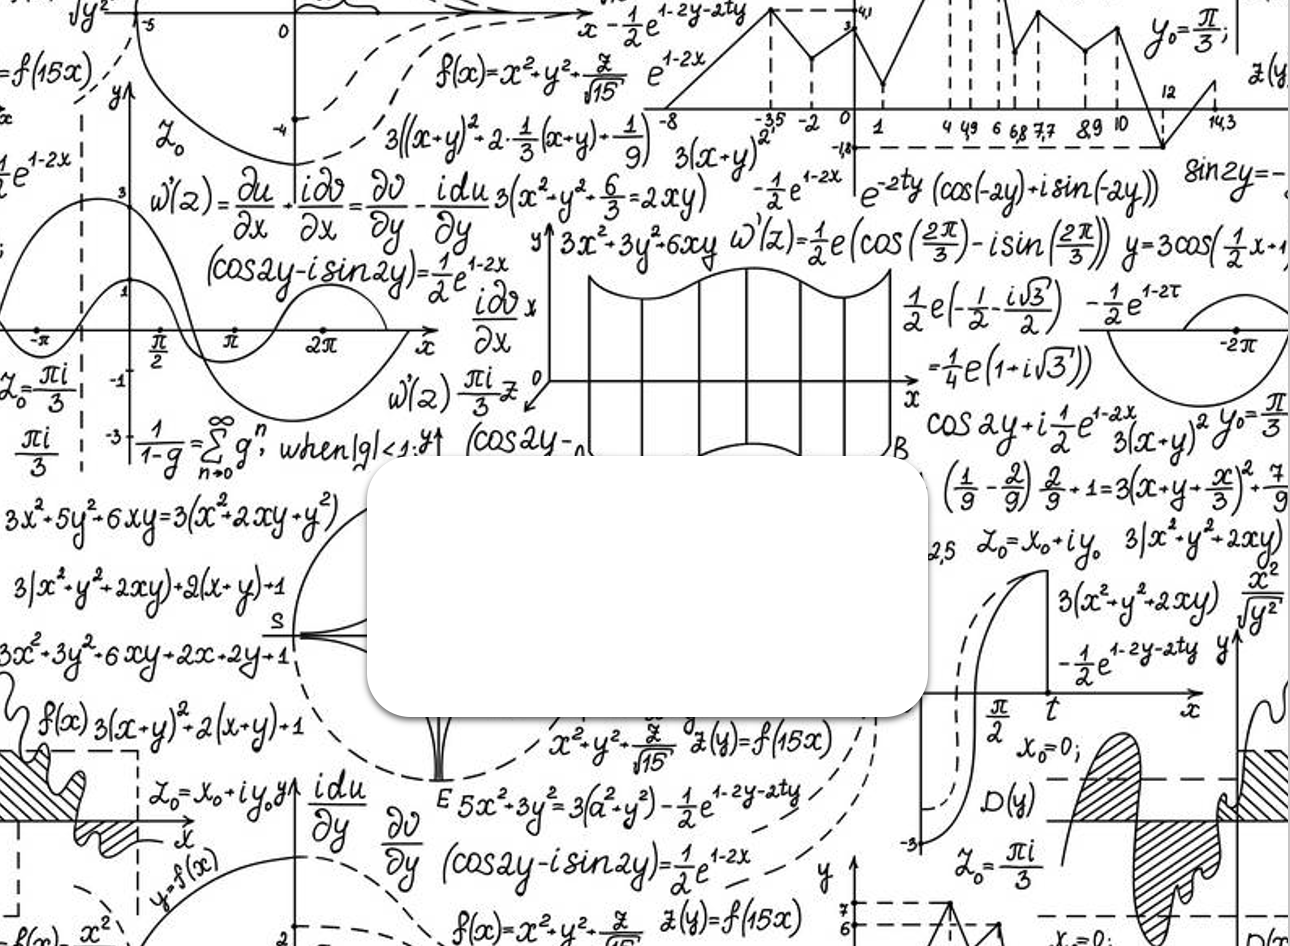
\includegraphics[width=\paperwidth,height=\paperheight]
{images/фон.png}}

\frame{\titlepage}

\setbeamertemplate{background canvas}{}

\begin{frame}

\frametitle{Оглавление}
\tableofcontents

\end{frame}

            
\section{Задание по геометрии с олимпиады}

\begin{frame}
\frametitle{Условие}
   \begin{Problem}
    Дан треугольник $ABC$, в котором $\angle A = \angle C =
    30^{\circ}$. \pause На его сторонах $AB$, $BC$ и $AC$
    выбраны точки $D$, $E$ и $F$ соответственно так, что
    $\angle BFD = \angle BFE = 60^{\circ}$. \pause Периметр
    треугольника $ABC$ равен $p$, а периметр треугольника
    $DEF$ равен $p_1$. \pause Докажите, что $p \leqslant
    2p_1$.
    \end{Problem}
\end{frame}


\subsection{Чертеж}

\begin{frame}{Чертеж}
\begin{figure}[h]
	\begin{center}
	\begin{tikzpicture}
	\draw (0, 0) -- (4,4) -- (8,0) -- (0,0);
	\draw[color=black] (4,4) -- (4,0);
	\draw[color=black] (3.5, 0) -- (3.5, 0.5) -- (4, 0.5);
	\begin{scriptsize}
		    \draw[color=black] (-0.5,0) node {$A$};
		    \draw[color=black] (4,4.5) node {$B$};
		    \draw[color=black] (8.5,0) node {$C$};
		    \draw[color=black] (-0.1,0.5) node {$D$};
		    \draw[color=black] (4,-0.3) node {$M$};
		    \draw[color=black] (4.7,-0.3) node {$F$};
		    \draw[color=black] (6.5,2) node {$E$};
		    
		 \end{scriptsize}
		 \draw[color=black, dashed] (0.5,0.5) -- (4.8,0);
		 \draw[color=black, dashed] (0.5,0.5) -- (6,2);
		 \draw[color=black, dashed] (6, 2) -- (4.8, 0);
		 \draw[color=black] (4, 4) -- (4.8,0);
	\end{tikzpicture}
	\caption{Чертеж}
  \end{center}
\end{figure}
\end{frame}

\subsection{Решение}

\begin{frame}
\frametitle{Решение}
\footnotesize

\begin{overlayarea}{\textwidth}{3em}

\only<1>{Пусть $\angle AFD = \alpha $. Поскольку угол $\angle BDF$ внешний для
треугольника $ADF$ , то $\angle BDF = \angle DAF + \angle AFD =  30^{\circ} +
\alpha$. Также $\angle BFA $ внешний для треугольника $BFC$,
поэтому $60^{\circ} + \alpha = \angle BFA = \line(1,0){50}$}

\only<2>{Пусть $\angle AFD = \alpha $. Поскольку угол $\angle BDF$ внешний для 
треугольника $ADF$ , то $\angle BDF = \angle DAF + \angle AFD =  30^{\circ} + 
\alpha$. Также $\angle BFA $ внешний для треугольника $BFC$,
поэтому $60^{\circ} + \alpha = \angle BFA = \textcolor{magenta}{\angle FBE + 
\angle FCB}$}

\only<3>{Следовательно, $\angle FBE = 30^{\circ} + \alpha = \angle FDB$ (см. 
рис. 2). Тогда, так как $\angle BFD = \angle BFE = 60^{\circ}$, треугольники 
$BDF$ и $EBF$ подобны.
Значит, $\frac{BF}{FE} = \frac{FD}{BF}$, или $BF^2 = FD \cdot FE$. Отсюда 
следует, что $DF + EF \geq 2\sqrt{DF \cdot EF} = 2BF$.}

\only<4>{По теорем косинусов для треугольника $DEF$ имеем: 

\[DE = \sqrt{DF^2 + EF^2 + DF \cdot EF} \geq \sqrt{2DF \cdot EF + DF \cdot EF}
= \line(1,0){50}\]}

\only<5>{По теорем косинусов для треугольника $DEF$ имеем: 

\[DE = \sqrt{DF^2 + EF^2 + DF \cdot EF} \geq \sqrt{2DF \cdot EF + DF \cdot EF}
= \textcolor{magenta}{BF \cdot \sqrt{3}}\]}

\only<6>{
Следовательно:

\[p_1 = DF + EF + DE \geq (2 + \sqrt{3}) \cdot BF.\]}

\only<7>{Пусть $BM$ - вычота равнобедренного треугольника $ABC$. Тогда легко 
увидето, что $p = (AB + BC) + AC = 4BM + 2\sqrt{3}BM = 2(2 + \sqrt{3})BM$. 
Осталось заметить, что $BF \geq BM$, поэтому $2p_1 \geq 2(2 + \sqrt{3})BF \geq 
2(2 + \sqrt{3})BM = p$. }

\end{overlayarea}
\end{frame}

\section{Контакты}

\begin{frame}
\frametitle{Контакты}
\framesubtitle{Как со мной связаться}
\begin{columns}[T] 
    \begin{column}{5cm} 
    \begin{itemize}
    \item<1-> \beamergotobutton{Телефон:}
    \item<2-> \href{https://t.me/at_one_day}{Telegram}
    \item<3-> \beamerskipbutton{Почта:}
    \end{itemize}
    \end{column}
    \begin{column}{5cm} 
        \centering
        
\includegraphics[height=3cm]{images/корги.jpg}
    \end{column}
\end{columns}
\end{frame}

\begin{frame}{Интерактив}
\frametitle{Интерактив}
\framesubtitle{Нажми на мой нос}
\framezoom< 1 >< 2 >[border = 4](5.1cm, 1.6cm)(1cm, 1cm) 
\centering

\includegraphics[height=4cm]{images/корги.jpg}
    
\end{frame}

\end{document}